% !TEX program = pdflatex
% !TEX enableSynctex = true
% !BIB program = bibtex

\documentclass[12pt]{article}

\usepackage{setspace}
\usepackage{amsmath}
\usepackage{amsfonts}
\usepackage{graphicx}
\usepackage{float}
\usepackage{dsfont}
\usepackage{natbib}
\addtolength{\oddsidemargin}{-.7in}
\addtolength{\evensidemargin}{-.7in}
\addtolength{\textwidth}{1.4in}
\usepackage{enumerate}
\onehalfspacing
\usepackage{geometry} % Required for customizing page layout
\usepackage{ragged2e}

\usepackage{caption}
\usepackage{booktabs}

\usepackage{hyperref}
\hypersetup{
	pdfstartview = FitH,
	pdfauthor = {...},
	pdftitle = {...},
	pdfkeywords = {...; ...; ...; ...},
	colorlinks = true,
	linkcolor = blue,
	urlcolor = blue,
	citecolor = blue,
	linktocpage=true
}

\DeclareMathOperator{\E}{\mathbb{E}}
\DeclareMathOperator*{\argmax}{arg\,max}
\DeclareMathOperator*{\argmin}{arg\,min}
\hbadness=10000

\title{Reorganizing Debt Finance toward \\ Cash Flow-Based Lending}
\date{}

\begin{document}

\author{Barnabás Székely}
\date{\today}
\vspace{-1in}

\maketitle

\begin{abstract}
\noindent

This paper studies asset-based and cash flow-based lending in a heterogeneous firms model, where bankrupt firms may file for liquidation or reorganization. Creditors impose stricter terms on cash flow-based debt contracts if the borrower is expected to liquidate under financial distress. This puts small firms at a disadvantage, as large reorganization costs often force the liquidation of these businesses. Since small firms also lack sufficient pledgeable assets, they have limited access to both loan-types. This yields misallocation of capital and aggregate productivity losses. However, regulations that facilitate the reorganization of small firms - such as the  U.S. Small Business Reorganization Act introduced in 2019 - can significantly reduce this source of misallocation, by improving access to cash flow-based debt.

\bigskip{}
\bigskip{}
%\bigskip{}
%\bigskip{}
%\vspace{-0.5cm}

Keywords: Heterogeneous firms, Credit market frictions, Cash flow-based lending, SME financing gap
\medskip{}
% JEL Classification Code: E32, C22, E27.
\end{abstract}
\thispagestyle{empty}

\pagebreak{}


\section{Introduction \label{sec:introduction}} 
Small and medium enterprises (SMEs) are often recognized as key drivers of job creation, innovation, and economic growth. Despite their importance, these firms regularly report difficulties in obtaining sufficient external finance (OECD, 2006). Given that small (young) firms typically lack sufficient collateral, borrowing against physical assets can provide them only limited access to external finance. Borrowing against future cash flows could offer a promising alternative, since this form of lending focuses on future earning potential rather than the accumulated collateral. However, as this paper argues, small firms' tendency to liquidate (rather than reorganize) under financial distress represents a significant limitation on their access to cash flow-based debt. \vspace{3mm} \\
Liquidation terminates all future cash flows, which drives lenders to impose stricter terms on cash flow-based debt contracts if the borrowers is expected to liquidate in default. This puts smalls firms at a disadvantage, since the legal and time costs of the reorganization process often force the liquidation of these businesses. Motivated by this dynamic, this paper studies the extent to which large reorganization costs exacerbate the SME financing gap, create misallocation of credit, and lead to a loss of aggregate productivity. Additionally, it evaluates regulations that aim to facilitate small firm reorganizations, such Small Business Reorganization Act\footnote{Small Business Reorganization Act (SBRA) introduced Subchapter V into Chapter 11 of the U.S. bankruptcy code in 2019. It aims to simplify and streamline the reorganization process for small businesses. See more detailed description in section \ref{sec:A2} the appendix. } for their potential to improve access to debt finance for small firms. \vspace{3mm} \\
The main contribution of this paper is a heterogenous firms model that consolidates structural models of bankruptcy resolution (Tamayo, 2017; Corbae and D'Erasmo, 2021) and market frictions associated with asset-based and CF-based lending (Drechsel, 2023; Öztürk, 2024; Gonzalez and Sy, 2024). Firms finance their investments by net wealth and borrowing against assets or future cash flows (Lian and Ma, 2021). A positive share of firms experience financial distress in equilibrium, which leads them to file for liquidation (Chapter 7) or reorganization (Chapter 11).
Reorganization allows firms to continue, but it incurs a fixed cost, which introduces economies of scale in the bankruptcy resolution process. Lenders set interest rates based on their exposure to default risk. In the case of CF-based contracts, the absence of physical collateral increases exposure liquidation risk. Hence, lenders must anticipate borrowers' bankruptcy resolution decisions and adjust the terms of the debt contract accordingly. As a result, firms that are expected to liquidate under financial distress may be shut out of the CF-based debt market entirely. \vspace{3mm} \\
This model is brought to the data using a combined dataset on US non-financial corporations and their debt financing strategies. The default resolution process is informed by a comprehensive dataset of US bankruptcy filings over the same period. The calibrated model suggests that... (\textit{add a description of results}) \vspace{3mm} \\
My analysis also presents a novel emphasis on the role of credit spreads in regulating borrowing behavior. Prior structural analyses of asset-based and cash flow-based lending impose borrowing limits such that firms always choose to meet their debt obligations. This yields `hard constraints' to borrowing: firms that borrow against assets are constrained by the value of their collateral, whereas those borrowing against cash flows are limited by current earnings. Since debt contracts are always honored under this framework, all firms face the same risk-free interest rate. As a result, prior structural analyses in this literature typically focus on debt covenants,\footnote{These are legally binding agreements imposed by the creditor on the lender, that typically take the form of hard constraints similar to those implied by the `no equilibrium defaults framework'.} while credit spreads receive considerably attention. \vspace{3mm} \\
The model presented in this paper, departs from this approach by also considering in-equilibrium defaults and default resolution decisions. This generates endogenous variation in the cost of external finance, as individual borrowers face different interest rates depending on their current state and debt financing decisions - i.e. `soft constraints' to borrowing. Therefore, this approach allows me to complement prior structural analysis by focusing on credit spreads rather than debt covenants. \vspace{3mm} \\
The structural analysis is also supported by an empirical analysis of debt contracts held by U.S. non-financial corporations between 2010 and 2023. This shows that size and profitability are important determinants of credit spreads for both type of debt contracts. This is in contrast with prior analyses that interpret credit market frictions as either asset-based or earings-based borrowing limits. Moreover, higher pledgeability of assets (defined as the share of collateralizable assets to total assets) is associated with lower credit spreads for asset-based debt but shows no significant impact on cash flow-based debt contracts. This is in line with the model prediction that lenders of CF-based debt consider the value of total assets as an indicator of liquidation probability rather than a direct determinant of in-default payoffs. \vspace{3mm} \\
The paper is organized as follows. Section 2 reviews the related literature. Section 3 addresses the empirical analysis, section 4 introduces the structural model framework, section 5 details the calibration of the model, and section 6 discusses the results. Section 7 concludes.

\section{Literature \label{sec:literature}} 
This paper contributes the most closely to the literature that separates asset-based and cash flow-based lending and considers their implications for credit market frictions. Corporate credit market frictions have traditionally been characterized as borrowing constraints defined the by value of pledgeable assets.\footnote{This dates back to the seminal works of Kiyotaki and Moore (1997) and Bernanke, Gertler, and Gilchrist (1999).} Recent research challenged this view based on more granular analyses of credit contracts. Most prominently, Lian and Ma (2021) finds that most of US corporate debt is backed by future cash flows rather than specific physical assets, suggesting that credit frictions are better described as earnings-based constraints. They support this by documenting the extensive use of earnings-based covenants in US corporate debt contracts. \vspace{3mm} \\
This result has prompted several studies to re-evaluate the role of credit market frictions in structural models. Drechsel and Kim (2022) argues that firms subject to earnings based constraints under-borrow, while those facing asset based constraints over-borrow. Drechsel (2023) demonstrates that the effects of investment shocks\footnote{There are exogenous shocks that move the price of the capital countercyclically.} are heterogeneous across firms depending on debt contract in place. Öztürk (2023) identifies quantitative differences in firms' reaction to a contractionary monetary shocks. He finds that asset-based borrowers experience sharper declines in borrowing and investment compared to cash flow-based borrowers. Gonzalez and Sy (2024) documents on Spanish data that reliance to CF-based borrowing (CF-based debt to total debt) is U-shaped across firms size. \vspace{3mm} \\
This study makes two distinct contributions to this literature. First, it considers equilibrium defaults and a liquidation decision, mostly drawing on Corbae and D'Erasmo (2021). This highlights liquidation risk as a key determinant of access to cash flow-based debt. Second, it deviates from prior structural analyses that impose borrowing limits, such that firms always meet their debt obligation. This assumption leads to `hard constraints' to borrowing where access to asset-based debt is limited by collateral value and cash flow-based borrowing is limited by current earnings. In contrast, considering equilibrium defaults yields `soft constraints' to borrowing, which  allows for the structural analysis of credit spreads in the context of asset-based and CF-based lending. \vspace{3mm} \\
I also contribute to the literature on credit market frictions and their role in capital misallocation and aggregate productivity losses (Banerjee and Moll, 2010; Buera, Kaboski, and Shin, 2011; Midrigan and Xu, 2014).\footnote{For a comprehensive review of the misallocation literature, see Restuccia and Rogerson (2012) and Hopenhayn (2014).} Even though the option to borrow against future cash flows could be expected to have a significant impact on credit allocation, few studies consider CF-based debt for quantifying misallocation caused by limited access to external finance (Gonzalez and Sy, 2024). This paper assesses productivity losses from misallocation in two distinct scenarios. In the baseline case, firms have access both asset-based and cash flow-based debt, but high reorganization costs often lead to the liquidation of small (young) firms. This is compared to a model calibration where reorganization costs are lower, limiting the liquidation risk of small firms. \vspace{3mm} \\
Finally, by highlighting liquidation risk as a major impediment to access to CF-based debt, this paper also contributes to the widespread literature on SME financing. For comprehensive overview of this literature see Esho and Verhoef (2018) and Rao et al. (2021). The majority of contributions in this literature assess specific policy programmes that aimed to enhance small firms' access to external finance, such as credit guarantee schemes and public-private partnerships. This paper argues that a bankruptcy framework supportive of small of reorganization may also improve small firms' access to CF-based debt finance. Moreover, it evaluates policies that facilitate small firm reorganizations (such the Small Business Reorganization Act) in light of this mechanism. 

\section{Empirical analysis \label{sec:empirical analysis}}
This section presents the empirical analysis of the debt financing strategies, and liquidation decisions of US non-financial corporations. Then, it explores the empirical determinants of credit spreads for asset-based and cash flow-based debt contracts. Finally, it provides indirect evidence that lenders consider the probability of liquidation when extending loans backed by future cash flows. \vspace{3mm} \\
I study a total of 113,774 debt contracts held by 6,925 non-financial corporations between 2010Q1 and 2023Q2. Debt-level data is provided by S\&P's Capital IQ and firm-level data is from Compustat North America. This yields and broad, but not representative sample of US non-financial corporations and their debt financing strategies. Moreover, I study Federal Judicial Center's Integrated Database (IDB), which contains a total of 160,367 Chapter 7 and Chapter 11 bankruptcy filings over the same period. Table 1. presents firm-level summary statistics for indicators of size, financial position, and borrowing conditions. Table 2. presents debt-level summary statistics, for contract value, maturity interest rates and spreads. 

\begin{table}[H] 
    \centering
    \resizebox{0.95\textwidth}{!}{%
    \begin{tabular}{lrrrrrr}
    \multicolumn{7}{l}{\textbf{Firm-Level Summary Statistics}} \\
    \hline
        & \textbf{Mean} & \textbf{p10} & \textbf{p25} & \textbf{Median} & \textbf{p75} & \textbf{p90} \vspace{1mm} \\
    Total Assets (millions USD) & 5235.16 & 11.39 & 73.11 & 582.60 & 2696.20 & 9567.60 \\
    Qtr. Revenue (millions USD) & 1073.75 & 0.18 & 8.77 & 109.62 & 551.79 & 1891.00 \\
    Employees (thousands) & 11.93 & 0.03 & 0.15 & 1.37 & 6.91 & 22.85 \\
    Firm Age (years) & 44.61 & 9 & 16 & 30 & 59 & 109 \\
    Cash to Assets (Liquidity) & 0.17 & 0.01 & 0.03 & 0.09 & 0.21 & 0.46 \\
    Debt to Assets (Leverage) & 0.30 & 0.03 & 0.12 & 0.27 & 0.43 & 0.61 \\
    Debt to Collateral & 0.51 & 0.11 &  0.26 &  0.52 & 0.75 & 0.89 \\ 
    Asset Pledgeability (\%) & 47.21 & 9.32 & 23.48 & 46.91 & 70.53 & 85.81 \\
    Total debt (millions USD) & 1817.35 & 1.06 & 8.33 & 132.69 & 960.90 & 3562.65 \\
    CF-share & 0.45 & 0.00 & 0.00 & 0.40 & 0.92 & 1.00 \\
    Average Maturity (years) & 6.7 & 1.4 & 4.0 & 6.1 & 8.6 & 12.2 \\
    Average Interest Rate (\%) & 4.9 & 0.3 & 2.7  & 4.6 & 6.8 & 9.2 \\
    Average Spread & 2.9  & 0 & 0.6 & 2.3 & 4.4 & 6.9 \\
    \hline
    \end{tabular}%
    }
    \caption{\small Summary Statistics - non-financial corporations between 2010Q1 and 2023Q2}
    \label{tab:sumstat}
\end{table}
\begin{table}[H]
    \centering
    \resizebox{0.95\textwidth}{!}{%
    \begin{tabular}{lrrrrrr}
    \multicolumn{7}{l}{\textbf{Debt-Level Summary Statistics}} \\
    \toprule
      	& \textbf{Mean} & \textbf{p10} & \textbf{p25} & \textbf{Median} & \textbf{p75} & \textbf{p90} \vspace{1mm}\\
    Contract Value (millions USD) & 334.53  & 0.16 & 2.24 & 48.24 & 396.00 & 859.22 \\ 
    Maturity (years) & 9.275 & 2.50 & 4.50 & 7.00 & 10.00 & 20.00 \\
    Interest Rate (\%) & 5.79 & 2.12 & 3.60 & 5.25 & 7.38 & 10.00 \\
    Credit Spread & 4.03  & 0.87 & 1.88 & 3.45 & 5.49 & 8.06  \\
	\bottomrule
    \end{tabular}%
    }
    \caption{\small Summary Statistics - debt contracts between 2010Q1 and 2023Q2}
    \label{tab:sumstat}
\end{table}

\noindent The classification strategy adopted here follows the principles outlined by Lian and Ma (2021) - this is described in detail in section \ref{sec:classification} of the appendix.  I find that $52.7\%$ of debt contracts can be classified cash flow-based. Since these are often large in terms of value, they collectively constitute 76.7\% of the total debt by volume - this aligns well with the aggregate values reported by Lian and Ma.\footnote{Nevertheless, it should be noted that due to data limitations, my approach is likely to yield a cruder classification, as I have considerably less data at my disposal.} The share of CF-based debt remains relatively stable (fluctuating within the range of 71.8\% to 79.8\%). However, it declines significantly in the year 2019 and remains subdued until the end of the sample period - see figure \ref{chart:CFLshare} in the appendix. 

\subsection{Determinants of Credit Spreads \label{sec:credit spreads}} 
In this section, I study the firm-level determinants of credit spreads for asset-based and cash flow-based debt contracts. As noted in the introduction, the structural model proposed in this paper accounts for endogenous variation in external finance premia, meaning that the empirical results presented here can be studied against predictions of the structural model. Credit spreads are calculated as the difference of the interest rate and the treasury rate at the corresponding maturity. To ensure that the observed credit spread reflects the original terms of the debt contract, I only consider the time of issuance. The regression analysis is carried out on sub-samples of asset-based and CF-based debt contracts as well as the entire sample and all specifications include period fixed effects. The results are summarized by table 3. \vspace{3mm} \\
Firms with higher EBITDA\footnote{For the estimation, I take the log-modulus transformation of of EBITDA values.} and larger total asset value benefit from lower credit spreads on both loan-types. Prior analyses that interpret credit market frictions as either asset-based or earings-based limits to borrowing. In contrast, this result suggests that size and profitability are important determinants of these frictions no matter the form of borrowing. Another important determinant of credit spreads is leverage, which has a large, positive effect on credit spreads for both loan-types. Firm age has a significant, negative effect on credit spreads, suggesting that strong creditor-debtor relationships can help reduce the cost of external finance.  \vspace{3mm} \\
The coefficient estimates for number of employees are not consistent across specifications. This variable has limited economic impact, which indicates that total assets is a sufficient measure of firms size. Consistent with the idea that lender perception plays a key role in cash flow-based borrowing, worse credit ratings significantly increase credit spreads for this type of debt. In contrast, credit spreads for asset-based debt are influenced only when credit ratings signal the state default or a high risk of it. Sector fixed effects have mostly insignificant impact on credit spreads for asset based debt, which is partly due to accounting for pledgeability in the model. For cash flow based debt, sector differences are more significant, yet they remain relatively unimportant determinants of credit spread variations. \vspace{3mm} \\
`CF share' measures the extent to which a firm relies on cash flow-based debt as a fraction of total debt. It is defined as 
\begin{equation*}
    \text{CF share} = \text{CF-based Debt Value} \  / \  \text{Total Debt Value}.
\end{equation*}
CF share is correlated negatively with spreads of cash flow-based debt and positively with spreads of asset-based debt, suggesting that firms self-select into these loan-types based on their relative costs. This underlines that debt financing is jointly determined with the credit spreads that firms eventually face. To give a complete account of firms' optimization, section \ref{sec:CFshare} in the appendix studies firm characteristics that influence firms' decisions on CF share.

\begin{table}[H]
    \centering
    \caption{The Determinants of Credit Spreads}
    \label{tab:spread_table_new}
    \resizebox{\textwidth}{!}{%
    \begin{tabular}{lcccccc}
    \toprule
    & \multicolumn{2}{c}{All contracts} & \multicolumn{2}{c}{CF contracts} & \multicolumn{2}{c}{AB contracts} \\
    \cmidrule(lr){2-3} \cmidrule(lr){4-5} \cmidrule(lr){6-7}
    \textbf{LHS}: Spread & Value & SE & Value & SE & Value & SE \\
    \midrule
    Log of EBITDA & -0.161*** & (0.0106) & -0.112*** & (0.0121) & -0.203*** & (0.0203) \\
    Log of Assets & -0.375*** & (0.0473) & -0.381*** & (0.0583) & -0.308*** & (0.0838) \\
    Pledgeability & -0.467*** & (0.0867) & -0.0297 & (0.108) & -0.990*** & (0.144) \\
    Leverage & 1.783*** & (0.103) & 2.278*** & (0.134) & 0.985*** & (0.168) \\
    Log of Age & -0.136*** & (0.0255) & -0.132*** & (0.0300) & -0.149*** & (0.0447) \\
    Log of Employees & -0.0118 & (0.0198) & -0.0974*** & (0.0252) & 0.0838*** & (0.0310) \\
    CF Share & 0.450*** & (0.0642) & -0.335*** & (0.112) & 0.748*** & (0.112) \vspace{3mm} \\
    \multicolumn{7}{l}{\textbf{Industries} - baseline: Agriculture and Fishing} \\
    Construction  & 0.739*** & (0.269) & 1.200*** & (0.461) & 0.275 & (0.375) \\
    Manufacturing  & 0.278 & (0.242) & 0.613 & (0.446) & 0.126 & (0.310) \\
    Mining & 0.847*** & (0.250) & 0.986** & (0.455) & 0.716** & (0.333) \\
    Retail Trade  & 0.677*** & (0.255) & 1.228*** & (0.455) & 0.0613 & (0.338) \\
    Services & 0.278 & (0.247) & 0.729 & (0.448) & -0.172 & (0.320) \\
    Public Utilities & 0.603** & (0.247) & 0.908** & (0.449) & 0.314 & (0.330) \\
    Wholesale Trade & 0.663** & (0.262) & 0.716 & (0.461) & 0.561 & (0.345)  \vspace{3mm} \\
    \multicolumn{7}{l}{\textbf{Credit Ratings} - baseline: Rating: A} \\
    Rating: A+ & 0.163* & (0.0928) & 0.391*** & (0.0857) & -0.417 & (0.568) \\
    Rating: A- &  0.170** & (0.0765) & 0.197*** & (0.0653) & -0.0652 & (0.361) \\
    Rating: B+ & 0.723*** & (0.0713) & 0.726*** & (0.0653) & 0.157 & (0.325) \\
    Rating: B & 0.213*** & (0.0679) & 0.140** & (0.0583) & -0.0439 & (0.329) \\
    Rating: B- & 0.986*** & (0.0718) & 1.180*** & (0.0687) & 0.206 & (0.323) \\
    Rating: C  & 1.711*** & (0.0812) & 1.679*** & (0.0896) & 1.108*** & (0.326) \\
    Rating: D & 2.023*** & (0.140) & 2.434*** & (0.185) & 1.073*** & (0.362)  \\
    \midrule
    Period fixed effects & Yes & & Yes & & Yes & \\
    Observations & 17,668 & & 10,676 & & 6,992 & \\
    R-squared & 0.286 & & 0.403 & & 0.173 & \\
    \bottomrule
    \multicolumn{7}{c}{Robust standard errors in parentheses} \\
    \multicolumn{7}{c}{*** p$<$0.01, ** p$<$0.05, * p$<$0.1} \\
    \end{tabular}%
    }
\end{table}


\subsection{Liquidation Risk and Credit Spreads \label{sec:emp liqprob}} 
The structural analysis suggests that in the case of cash flow-based debt, the ex-ante liquidation probability is an important determinant of credit spreads. Although this variable is not directly observable, the empirical analysis suggests that it is taken into consideration by creditors. Table 3. shows that the credit spread decreases with total assets for both loan-types. In the case of asset-based debt, pledgeability\footnote{Defined as the proportion of collateralizable assets to total assets - see precise variable definitions in section \ref{sec:A3} of the Appendix.} also has a considerable negative effects on credit spreads. However, for CF-based debt contracts it remains insignificant, indicating that for these contracts lenders do not value assets as collateral. Rather, they view firm size (measured by the value of assets) as an intrinsic advantage. \vspace{3mm} \\
Figure 1 shows that the probability of liquidation under financial distress decreases sharply with firms size. Hence, this finding supports the idea that for cash flow-based debt, lenders consider the value of total assets as an indicator of liquidation probability rather than a direct determinant of in-default payoff. An alternative explanation could be that larger firms’ superior accounting practices help reduce information asymmetries between borrowers and lenders. However, the model controls for firm age, which often regarded as the most important determinant of information frictions. Additionally, the inclusion of credit ratings, which are likely a key determinant of creditor perceptions, further weakens this point.
\begin{figure}[H]  % [h] indicates placing the image here
    \centering  \label{chart:mixplot}
    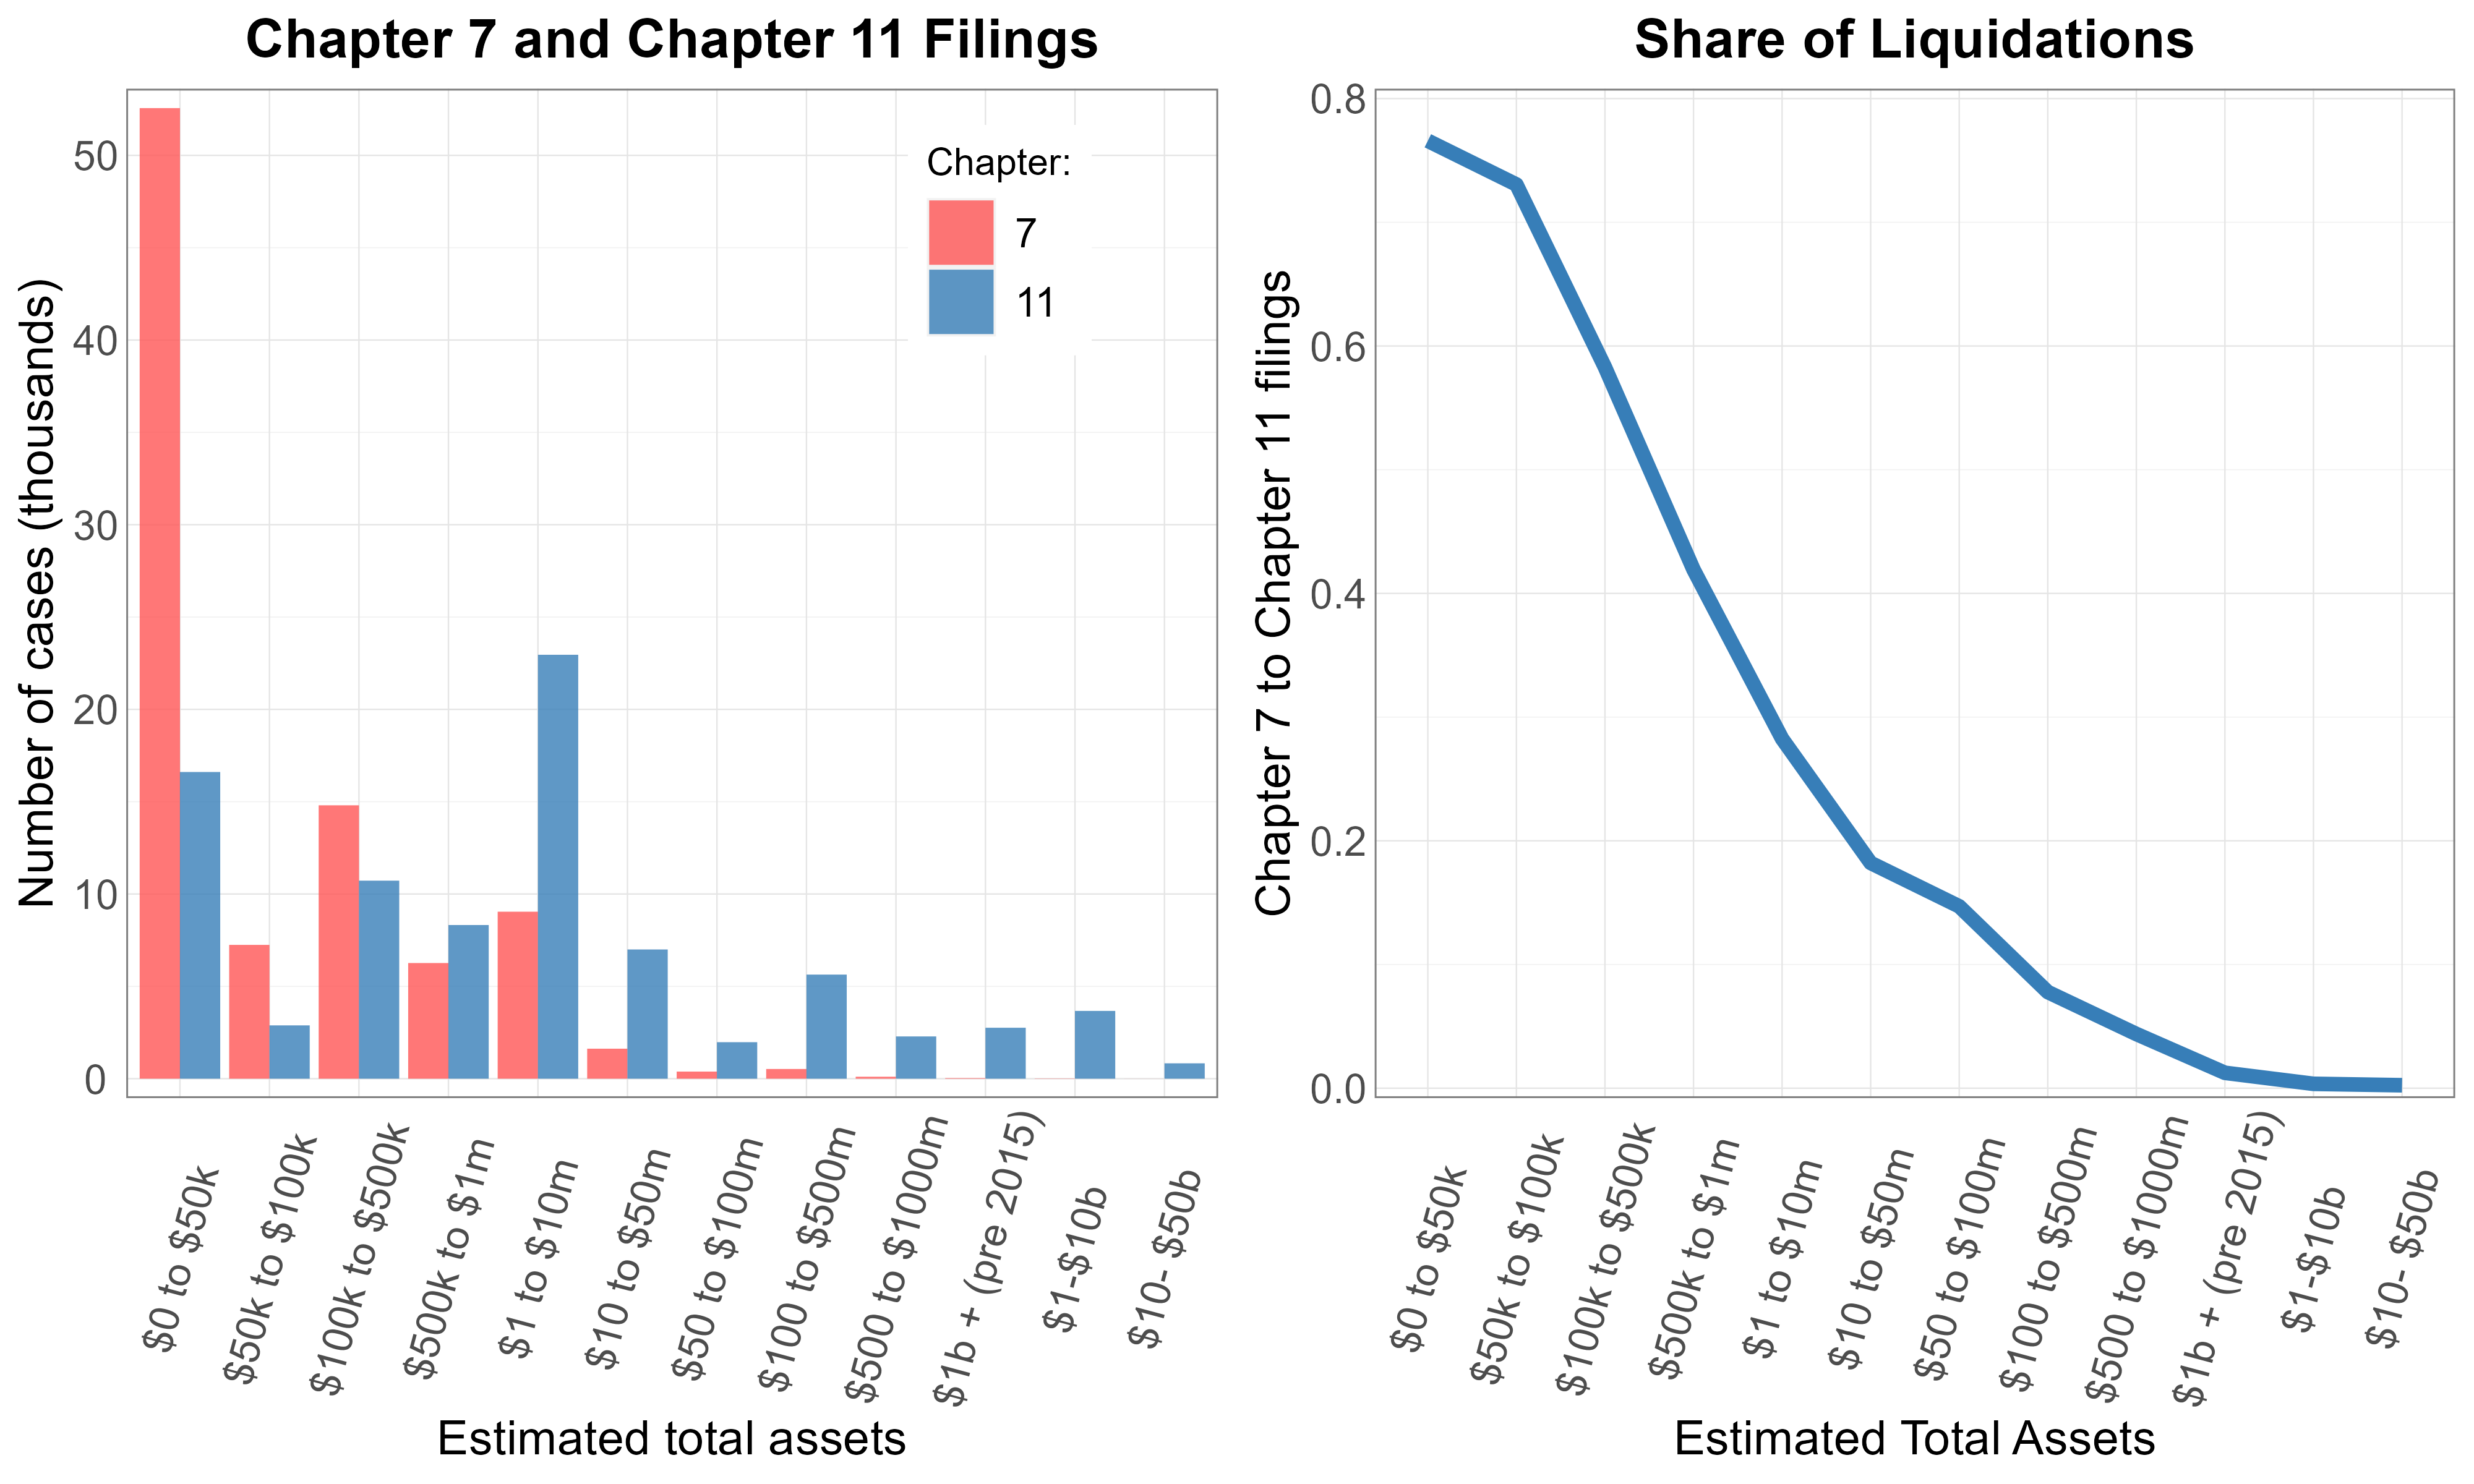
\includegraphics[width=1\textwidth]{C:/Users/szjud/OneDrive/Asztali gép/EBCs/CFL-git/Latex codes/Plots/liqprob2.png}
    \footnotesize \justifying Panel A. shows the all chapter 7 and 11 instances between 2010 and 2023 across firm sizes. Panel B. shows the proportion of chapter 7 filings as a share to total bankruptcies. 
\end{figure}


\subsection{Robustness and Limitations \label{sec:limitations}} 
I test the robustness of these results in alternative model specifications - these are published in section \ref{sec:robustness} of the appendix. Since, calculating credit spreads is subject to uncertainty, the analyses presented in table 3 are repeated with interest rate as the dependent variable - in this case, maturity is also considered in the regression. Moreover, limiting the analysis to new issuances reduces the sample size. By using a weighted average of firm-level credit spreads as the outcome variable, it is possible to explore the variables that influence external finance premia beyond the time of issuance. Here, I consider three sub-samples: firms with CF share over 90\%, less than 10\% and all firms. The central findings of this section remain largely unchanged across all specifications. \vspace{3mm} \\
Empirical analyses of credit spreads and firm characteristics face significant limitations. Firms adjust their debt financing strategies based on credit conditions, which are influenced by firm characteristics. In turn, this affects the external finance premia they eventually face. This, in all likelihood, introduces considerable endogeneity bias. Moreover, certain determinants of credit frictions are difficult to observe. In this paper, I highlight the probability of liquidation as an important determinant. However, other factors such as assets specificity (Kermani and Ma, 2020) or the quality of accounting practices and court enforceability (Lian and Ma, 2021) are similarly hard to measure. Therefore, identification of causal relationships between firm characteristics and credit spreads is not possible without relying on natural experiments. The structural model discussed below aims to make up for these limitations. 

\section{Model outline} \label{sec:model}
This section introduces a discrete-time general equilibrium model with firms that are heterogeneous in productivity, own capital and may borrow against assets or cash-flows. Firms may experience financial distress, which is resolved either through liquidation or reorganization. Reorganization incurs a fixed costs, making larger firms better positioned to avoid liquidation in default. The competitive lender must adjust the terms of the debt contract accounting for credit risk. CF-based debt is not secured by physical collateral, meaning that it exposes the lender to liquidation risk. Finally, the representative household that provide an inelastic labour supply, chooses a stream of consumption and one-period, noncontingent bonds to maximize expected discounted utility. 
\subsection{Heterogenous Firms \label{sec:firms}}
Firms produce a homogeneous consumption good, using labour $n$ and capital $k$, with a decreasing returns to scale production technology:
\begin{equation} \label{eq:prodf}
y = \varepsilon k^{\alpha}n^{\nu}, \ \ \ \ \alpha,\nu \in (0,1),  \ \nu + \alpha \in (0,1)
\end{equation}  
where $\varepsilon$ is the idiosyncratic productivity state. In the interest of keeping the notation simple, I omit firm subscripts. \vspace{3mm} \\
Firms own capital and investments are financed partly by retained earnings and partly by borrowing from a competitive lender. At any given period, a firm can be described by the predetermined capital stock $k \in \mathbf{K} \subset \mathbf{R^{+}}$, debt $b \in \mathbf{B} \subset \mathbf{R}$ and current productivity $\varepsilon \subset \mathbf{R^+}$.  Idiosyncratic productivity is a Markov chain on the finite set $\varepsilon \in \mathbf{E} \equiv \{ \varepsilon_1,...,\varepsilon_{N_{\varepsilon}} \}$ such that $ g_{ij} \equiv \Pr(\varepsilon'= \varepsilon_j|\varepsilon = \varepsilon_i) \geq 0$ and $\sum_{j=1}^{N_{\varepsilon}} g_{ij} = 1$ for each $i$. Moreover, it is stochastically monotone such that for any fixed $x$, $\Pr(\varepsilon' \leq x | \varepsilon = \varepsilon_i)$ is decreasing in $\varepsilon_i$. The distribution of firms can be summarized using the probability measure $\mu$ defined on the Borel algebra $A$, generated by the open subsets of the product spaces $ \mathbf{A} = \mathbf{K} \times \mathbf{B} \times \mathbf{E} $.

\subsubsection{Labour Demand and Production \label{sec:labour demand}}
Production occurs before the realization of exit and entry decisions, and optimal labor demand is independent of current debt. Therefore, at the beginning of the period every firm of state vector $(k,\varepsilon)$ faces the same static optimization with respect to labour: 
$$ \pi(k,\varepsilon) = \max_{n} \ \  \varepsilon k^{\alpha}n^{\nu} - wn - c$$
where $c$ is a fixed cost of participating in production, $w$ is the wage and the price of the consumption good is flexible and normalized to $1$. Optimization yields the policy function for labour demand, $n(\varepsilon,k)$ and optimal production $y(\varepsilon,k)$: 
\begin{equation} \label{eq:opt_emp_prod}
n(k,\varepsilon) = \left( \dfrac{ \nu \varepsilon k^\alpha}{w} \right)^{\frac{1}{1-\nu}} \hspace{15mm}
y(k,\varepsilon) = \varepsilon k^{\alpha} \left( \dfrac{\nu \varepsilon k^\alpha}{w} \right)^{\frac{\nu}{1-\nu}}.
\end{equation}  
Firm profit function can be reformulated as: 
\begin{equation} \label{eq:profit}
\pi(k,\varepsilon) = y(k,\varepsilon) - wn(k,\varepsilon) - c = (1-\nu) y(k,\varepsilon) - c.
\end{equation} 
Firms own capital and make investment decisions, subject to a capital accumulation function,
\begin{equation} \label{eq:capital}
k' = (1-\delta)k + i
\end{equation} 
where $\delta$ is the depreciation rate and $i$ is investment. Since capital and debt are free of adjustment costs, the financial position of firms can be summarized by the cash on hand variable:
\begin{equation} \label{eq:cash on hand}
    x = \pi(k,\varepsilon) + (1-\delta)k - b.
\end{equation}

\subsubsection{Firm Values} \label{sec:Firm Values}
Production takes place at the beginning of the period. Firms set their labour demand given $(k,\varepsilon)$, profits are realized and capital depreciates. Then, incumbents may decide to exit, default or continue production to the next period. This decision is governed by: 
\begin{equation} \label{eq:default decision}
    V(k,b,\varepsilon) = \max \{V_{def}, \  V_{exit}(k,b,\varepsilon),  \ V_{cont}(k,b,\varepsilon) \}.
\end{equation}
Default is associated with zero value to the firm. This assumption implies that changes in the cost of reorganization only affects firm values through access to debt finance.\footnote{It also serves a practical purpose as it keep the computation burden of the model manageable.}
\begin{equation}
    V_{def} = 0.
\end{equation}
Moreover, firms may decide to exit after repaying their debt debt obligations. This allows firms to retain the value of the undepreciated capital stock net of debt service: 
\begin{equation}
    V_{exit}(k, b, \varepsilon) = \pi(k,\varepsilon) + (1-\delta)k - b  = x.
\end{equation}
Firms that decide to continue can obtain external financing through one-period debt contracts. For each unit of debt due in the next period, they receive $q$ units of output, which can be used towards investment or distributed as dividends. Moreover, continuing firms decide what proportion of their debt to be backed by future cash flows. In the following, I refer to this as the debt financing strategy of the firm and it is summarized by $\tau \in [0,1]$, where $\tau$ measures the value of CF-based to total debt - analogously to the `CF share' introduced in the empirical analysis. \vspace{3mm} \\
Continuing firms choose future capital stock $k'$, total future debt $b'$, and debt financing strategy $\tau'$ to maximize the discounted sum of dividends $d$, 
\begin{equation} \label{eq:dividends}
d = x - k' +  q(k',b',\varepsilon, \tau')b'.
\end{equation} 
Since capital and debt are not subject to adjustment costs, firms' financial position can be summarized by the cash on hand variable defined in equation \ref{eq:cash on hand}. This reformulation is reduces the computational burden of the model. Using the cash on hand variable, the value of continuation can be described as,
\begin{equation} \label{eq:V_cont}
    V_{cont}(x,\varepsilon) = \max_{k',b', \tau'} \left(x - k' +  q(k',b',\varepsilon, \tau')b' + q_f \E_{\varepsilon'|\varepsilon} V(k',b', \varepsilon') \right)
\end{equation}
subject to: 
\begin{equation} \label{eq:budget}
x' = \pi(k',\varepsilon')+(1-\delta)k'-b' \hspace{5mm} \text{and} \hspace{5mm} d \geq 0
\end{equation} 
where $q_f$ is firms' subjective discount factor. Note that since firms are owned by the household, future dividend payments are discounted using the household's discount factor, $\beta = q_f$.  \vspace{3mm} \\
Finally, entrants are endowed with zero starting cash on hand, reflecting that startups are typically asset-poor. These firms do not produce in the first period, and have the option to exit after drawing an initial productivity value. Hence, their initial decision can be described as: 
\begin{equation} \label{eq:entrant decision}
    V_e(\varepsilon) = \max \{0,  \ V_{cont}(0,\varepsilon) \}.
\end{equation}
That is, potential entrants solve \ref{eq:V_cont} - \ref{eq:budget} similarly to continuing firms, with the difference that their cash on hand is exactly zero. If $V_{cont}(0,\varepsilon)$ is smaller than zero, they exit voluntarily, without ever participating in production.

\subsubsection{Firm dynamics}
Firms may default endogenously, based on the decision rule specified in \ref{eq:default decision}. Additionally, they may experience an exogenous default shock, which reaches all firms with a uniform probability $P_{x}$ - this shock is necessary to calibrate the share of reorganizations to the data. To describe firm dynamics, I define the following indicator function. Let $\chi_{d} = 1$ if the firm defaults either due to endogenous decisions or the exogenous shock, $\chi_l = 1$ if the firm is liquidated in default (this decision is further discussed in section \ref{sec:default resolution})  and let $\chi_{ex} = 1$ if the firm exits voluntarily, after fulfilling its debt obligations. \vspace{3mm} \\
Voluntary exits and liquidations are balanced by a mass $M$ of potential entrants. Entrants' initial productivity is drawn from the stationary distribution of the Markov chain that defines idiosyncratic productivity - this is denoted by $\Phi(\varepsilon)$. Finally, let $\mu_0$ be the measure of the mass of firms at the beginning of the period. Taking stock movements on the extensive margin, the measure of firms at the end of the period can be expressed as: $\mu = (1 - \chi_l - \chi_{ex}) \mu_0  + (1 - \chi_{ex}) M d \Phi(\varepsilon) $. \vspace{3mm} \\
The evolution of firm distribution satisfies: 
\begin{equation} \label{eq_firmdim} 
    \mu_{0}'(A) = \int \mathbf{I}_{(k', b', \varepsilon') \in A} g(\varepsilon'|\varepsilon) \ d \mu (k,b,\varepsilon)
\end{equation}
for all Borel sets $A \subset  \mathbf{K} \times \mathbf{B} \times \mathbf{E} $ and where $g(\varepsilon'|\varepsilon)$ is the transition probability matrix idiosyncratic productivity. Finally, I summarize the dynamics of firm distribution at the beginning of the period by the mapping $ \mu'_0 =\Gamma(\mu_0)$.


\subsection{Households}\label{sec:hh}
\subsubsection{Consumption and Savings Decision} \label{sec:Cons and Savings decision}
There is a unit measure of identical households that choose a stream of consumption $C$ and one-period, noncontingent bonds $B$ which yield the risk free interest rate $q_0$ to maximize expected discounted utility. Households take firm measure $\mu_0$ as given. Their problem can be defined recursively as: 
\begin{equation} \label{eq:U_max}
V_h(B, \mu_0) = \max_{C,B'} U(C) + \beta V_h(B',\mu_0')
\end{equation}  
subject to: 
\begin{equation} \label{eq:const_hh}
C + B + \leq w N^s + q_0 B' + T
\end{equation} 
where $N^s$ is the inelastic labour supply, $\beta$ is the households' discount factor and $T$ denotes expenses and revenues from the production sector, shared within the household. Revenues include dividends from continuing firms and net wealth from exiting firms, while expenses cover the costs of reorganizing firms:
\begin{equation} \label{eq:T}
    \begin{split}
        & T = \int (1 - \chi_l - \chi_{ex}) \left( x - k'(k,b,\varepsilon) + qb'(k,b,\varepsilon) \right) d \mu_0(k,b,\varepsilon) \\
        & \qquad + \int \chi_{ex} \ x \ d \mu_0(k,b,\varepsilon) - \int \chi_d (1-\chi_{l}) \ \min\{b, \ \phi_c V_{cont}(k,b, \varepsilon) \} \ d \mu_0(k,b,\varepsilon).
    \end{split}
\end{equation}

\subsubsection{Default Resolution Decision} \label{sec:default resolution}
Default can be resolved through liquidation or reorganization. In the case of liquidation, the firm exits, and \textit{all} its undepreciated capital stock is resold at a discounted value, $\phi_l(1-\delta)k$, where $\phi_l \in (0,1)$. The rest of the stock cannot be recovered by the household, which indicates that corporate assets are often highly specialized and illiquid, which reduces their reusability (Kermani and Ma, 2020). The proceeds from this sale are distributed to the lender, who cannot recover an amount exceeding the value of the debt. Thus, the value of liquidation for the household is given by:
\begin{equation}
    V_{l}(k, b) = \max \{ 0, \ \phi_l(1-\delta)k - b  \}.
\end{equation}
In the case of reorganization, the household pays a fraction $\phi_c$ of the continuation value to the lender. This transfer represents the renegotiation of the debt contract, meaning that it cannot exceed the initial value of the debt. Hence, the household pays, $\min\{b, \ \phi_c V_{cont}(x,\varepsilon) \}$. Moreover, reorganization incurs a fixed cost $\zeta_r$ which is borne entirely by the household.\footnote{The incidence of the fixed cost has a minimal effect credit market frictions. Lenders' expenses directly raise the external finance premium, whereas borrowers' costs limit access to external finance indirectly by raising liquidation risk.} On the flip side, reorganization allows the firm to continue into the next period, which is of $V_{cont}(k,b,\varepsilon)$ value to the household. Taking stock, the value the household associates with reorganizing the firm is: 
\begin{equation}
    V_{r}(k, b, \varepsilon) = V_{cont}(k,b,\varepsilon) - \min\{b, \ \phi_c V_{cont}(k,b,\varepsilon) \} - \zeta_r.
\end{equation}
The liquidation decision amounts to choosing the option that allows the household to retain the most value. The indicator function $\chi_l$ can therefore be defined as:
\begin{equation} \label{eq:liquidation decision}
    \chi_l =  \mathds{1}( V_l(k, b)  \ \geq \ V_r(k, b, \varepsilon) \ | \ \chi_{D} = 1)  
\end{equation}
This highly stylized description  of the default resolution process effectively captures the decreasing liquidation probability across firm sizes. It should be noted however, that in practice this process typically involves negotiations between the borrower and multiple creditors, under the oversight of courts. For more realistic depictions of the bankruptcy process, see Tamayo (2017) and Hu and We (2018). \vspace{3mm} \\
Next, I describe the financial intermediation and the determinants of firms optimal debt financing strategy. To simplify notation, I summarize the collection of decision variables as $a = (k, b, \tau) $ in the following. 

\subsection{Financial Intermediation}  \label{sec: Financial Intermediation}
\subsubsection{The lender's problem}    \label{sec: The lender's problem}
The opportunity cost of lending to firms is determined by the risk-free bond yield $q_0$. However, since corporate lending is subject to default risk, the competitive lender must charge a premium to break even. When setting $q(a',\varepsilon)$ the lender must consider the expected payoff under 3 distinct scenarios: \textit{a)} orderly repayment; \textit{b)} the firm defaults and is liquidated \textit{c)} the firm defaults and is reorganized. It follows from the zero-profit condition that the debt schedule offered to firms is, 
\begin{equation} \label{eq:q}
    \begin{split}
        & q(a', \varepsilon)b' = q_0 \left[ \left(1-P_D(a', \varepsilon)\right)b' + \right. \\
        & \qquad P_D(a', \varepsilon) \gamma(a', \varepsilon) \min \{b', \ \Pi_{l}(a')\} + \\ 
        & \qquad \left. P_D(a', \varepsilon) (1-\gamma(a', \varepsilon))\min \{b', \ E_{\varepsilon' | \varepsilon} [ \Pi_{r}(a', \varepsilon') |\chi_r = 1 ] \} \right]
    \end{split}
\end{equation}
where 
\begin{itemize}\setlength\itemsep{0em} 
    \item $\Pi_{l}(a')$ is the expected payoff if the firms undergoes liquidation,
    \item $\Pi_{r}(a', \varepsilon)$ is the expected payoff if the firms undergoes reorganization,
    \item $P_D(a', \varepsilon)$ is the probability of default,
    \item $\gamma(a', \varepsilon)$ is the probability of liquidation under financial distress. 
\end{itemize} 
In the following, I discuss the determinants of these values. This yields a complete description of the debt schedule $q(a', \varepsilon)$.
 
\subsubsection{Lenders' In-default Payoffs, Given Debt Contract}   \label{sec:Default Resolution}
This section describes lenders' expected, in-default pay-offs when debt is backed by physical assets or by future cash flows. These pay-offs are central to the analysis as they shape the debt schedule $q(a', \varepsilon)$, that firms must consider in choosing debt financing strategy. The model considers two loan types (asset-based and cash flow-based) and two bankruptcy types (liquidation and reorganization), therefore the lender has four distinct cases to consider. \vspace{3mm} \\
\textit{ 1.) The recovery of asset-based debt when the firm undergoes liquidation}. Since the debt contract is backed by physical assets, the lender can recover the entire liquidation value of the firm, $\phi_l(1-\delta)k$. Note that this case corresponds to the traditional assumption on lenders' in-default payoffs.  \vspace{3mm} \\
\textit{ 2.) The recovery of asset-based debt when the firm undergoes reorganization}. When the borrower undergoes reorganization secured lenders are protected by the ‘best interest of creditor’ test.\footnote{The EU Directive refers this principle as ‘best-interest-of-creditors’ test in OJ L 172/27, art. 49; whereas the US bankruptcy code establishes this principle in - see section \ref{sec:A1} in the appendix} This states that creditors cannot be worse off under the reorganization plan than they would be under of liquidation. Therefore, I assume that the lender can retrieve the same $\phi_l(1-\delta)k$ as they would under liquidation. Theoretically this value could be higher, but it unlikely that the lender would expect to retrieve more than the value of the collateral backing the debt contract. \vspace{3mm} \\
\textit{ 3.) The recovery of CF-based debt when the firm undergoes liquidation}. In this case, the debt is not backed by physical collateral, which makes the lender ill-equipped to recover the liquidation value.  As a result, the lender can only recover a fraction $\kappa$ of the total liquidation value, $\phi_l(1-\delta)k$, where $\kappa$ is close to zero. \vspace{3mm} \\
\textit{ 4.) The recovery of CF-based debt if the firm undergoes reorganization}. In this case, the lender can claim a fraction of the continuation value such that its payoff is $\phi_c V_{cont}(x,\varepsilon)$. Hence, in this case the lender's payoff is determined by the continuation value of the firm.\footnote{For an analogous description of lenders in-default payoffs, see Drechsel (2023) - he demonstrates that with no equilibrium defaults, this yields earnings based borrowing constraints.} In practice, this process may vary depending on specifics of the debt contract. When the debt is secured against the entire corporate entity, the lender may gain access to borrower's cash flows directly. When the debt is unsecured, higher continuation value of the firm allows the lender to negotiate better terms during reorganization. For a detailed description of this mechanism see Corbae and D'Erasmo (2021). \vspace{3mm} \\
Table \ref{tab:lender payoffs} summarizes the payments extended by the household, the value the lender can seize given the debt contract that is in place. To keep the model simple, I assume that whatever the lender cannot seize due to contracting frictions is the welfare loss of the default resolution process. 
\begin{table}[h!]
    \centering
    \begin{tabular}{lccc}
         & Household's costs & Lender's payoffs & Welfare Loss \\
       \midrule
      AB debt, Liquidation & $ \phi_l (1-\delta) k$ &  $ \phi_l (1-\delta) k$ &  $ (1-\phi_l) (1-\delta) k$ \\
      AB debt, Reorganization &   $\phi_cV_{cont}(x,e)$  &  $ \phi_l (1-\delta) k$ &   \\
      CF debt, Liquidation & $ \phi_l (1-\delta) k$ &  $ \kappa \phi_l (1-\delta) k$ &   \\
      CF debt, Reorganization & $\phi_cV_{cont}(x,e)$ & $ \phi_c V(x,\varepsilon)$ &  \\ 
     \bottomrule
     \end{tabular}
    \caption{\small The lender's payoffs under each default resolution, debt contract pair gross of fixed costs.} 
    \label{tab:lender payoffs}
\end{table}

\noindent Table \ref{tab:lender payoffs} captures the central trade-off of lending against future cash flows or physical assets. When debt is asset based the lender may expect to retrieve the liquidation value of the firm, irrespective of the default resolution. In contrast, when debt is CF-based the lender expects to retrieve a share of the continuation value under reorganization, but risks losing out if liquidation occurs.

\subsubsection{Lenders' In-default Payoffs, Given Debt Financing Strategy}   \label{sec:Default Resolution}
It is now possible to outline the lender's expected payoff depending on debt financing strategy adopted prior to bankruptcy. Recall that the share of CF-debt to total debt is defined by $\tau \in (0,1)$. Hence, the lender's payoff under liquidation (or reorganization) is a linear combination of the payoffs from asset-backed debt (with weight $\tau$) and CF-debt (with weight $1-\tau$). \vspace{3mm} \\
First, consider debt-recovery under liquidation. The liquidation value of the firm is: $\phi_l (1-\delta) k$. However, the lender can only retrieve this value for the debt that is backed by physical assets, which is $1-\tau$ share of the total debt. After the remaining $\tau$ share, which corresponds to CF-based debt, the lender can seize only $\kappa$ fraction of original liquidation value - see top-left and bottom-left of table \ref{tab:lender payoffs}. Taking stock, the if the borrower is liquidated the lender receives:\footnote{Note that this value might be smaller than what is taken from the firm in case of liquidation. For the sake of simplicity, I assume that the difference of the two is a welfare loss of the liquidation process.}  
\begin{equation} \label{eq:P_liq} 
   \Pi_{l}(a) = (1-\tau) \phi_l (1-\delta) k +\tau \kappa \phi_l  (1-\delta) k. 
\end{equation}
When the firm undergoes reorganization the lender can claim a fraction of future cash flows after CF-based debt. Moreover, in accordance with the `best interest of creditor test' the lender expects to retrieve a payment that is equal to the liquidation value of the collateral after asset-based debt - see bottom-right and top-right of table \ref{tab:lender payoffs}. Hence, when the borrower undergoes reorganization, the lender receives
\begin{equation}  \label{eq:P_reorg}
   \Pi_{r}(a,\tau) = (1-\tau) \phi_l (1-\delta) k +\tau \phi_c V_{cont} (x, \varepsilon).
\end{equation}
Finally, the probability default and liquidation can be defined using the indicator functions introduced in section \ref{sec:defaults}: 
\begin{equation} \label{eq:default probability}
    P_D(a',\varepsilon) = \E_{\varepsilon'|\varepsilon}[\chi_l(a',\varepsilon') + \chi_r(a',\varepsilon')],
\end{equation}
and
\begin{equation} \label{eq:liquidation probability}
    \gamma(a',\varepsilon) = \E_{\varepsilon' |\varepsilon}[\chi_l(a',\varepsilon')].
\end{equation}
Bringing default and liquidation probability (equation \ref{eq:default probability} and \ref{eq:liquidation probability}) and expected payoff under liquidation and reorganization (equation \ref{eq:P_liq} and \ref{eq:P_reorg} respectively) to the zero profit condition described in equation \ref{eq:q} yields a complete description of the debt schedule $q(a', \varepsilon)$ offered to firms. Firms choose the debt financing strategy that maximizes the continuation value as described in equation \ref{eq:V_cont} - \ref{eq:budget}.

\subsection{Stationary equilibrium}\label{sec:eq}
The stationary competitive equilibrium is described by the set of functions
$$(\mu_0, \mu, w, V, V_{cont}, V_{def},  V_{exit}, V_r, V_r, \chi_l, \chi_l, \chi_{ex}, n,k,b,d,\tau,q, C, B)$$
such that: 
\begin{enumerate}[(i)]
\item households solve utility maximization: $V_h$ solves \ref{eq:U_max}-\ref{eq:const_hh} and the associated policy functions are $(C, B)$;
\item the lender solves \ref{eq:q} such that $q(a',\varepsilon)$ yields zero profits in expectation on each debt contract;
\item firms solve value maximization: $V$ solves \ref{eq:default decision}, $V_{def}$ solves \ref{eq:liq or reorg} and $V_{cont}$ solves \ref{eq:profit}, \ref{eq:V_cont} and \ref{eq:budget}; and the associated policy functions are $n$, for exiting and defaulting firms and $(n,k,b,d,\tau,q)$ for continuing and entering firms;
\item wages adjust to equate firms' labour demand to the inelastic labour supply
$$ N^s = \int n  \ d \mu_0 (k,b,\varepsilon)  $$
\item the first order condition households' savings problem implies that the interest rate of the noncontingent bond $q_0$ is equal to households' discount parameter $\beta$; and the financial market clears at $q_0 = q_f = \beta$
 $$ B = \int b \ d \mu_0 (k,b,\varepsilon) $$
\item goods market clears due to Walras' law (binding budget constraints and all other markets are in equilibrium) and aggregate consumption is
 $$ C = Y - I - \Psi$$
where
 $$ Y =  \int y \ d \mu_0 (k,b,\varepsilon) $$
aggregate investment is the sum of investment carried out by continuing incumbents and entering firms minus the capital freed up due to liquidations and voluntary exits:
\begin{multline*} 
    I = \int   k' -(1-\delta)k \ d \mu (k,b,\varepsilon) + M \int (1-\chi_{ex}) k' \ d \Phi(\varepsilon)    \\
   -  \int   \chi_l \phi_l (1-\delta)k \ d \mu_0 (k,b,\varepsilon) - \int \chi_{ex} (1-\delta) k \ d \mu_0 (k,b,\varepsilon)   
\end{multline*}
$\Psi$ collects the fixed costs of operation and the costs of financial intermediation\footnote{!Might need an additional term here, for liquidations where $\tau \neq 0$}
$$ \Psi = \int  \chi_l (1-\phi_l) (1-\delta)k \ d \mu_0 (k,b,\varepsilon) + \int  \chi_r \zeta_r \ d \mu_0 (k,b,\varepsilon) + \int  c \ d \mu_0 (k,b,\varepsilon) $$
\item the distribution measure of firms is stationary, $\Gamma(\mu_0) = \mu_0$ and prices $(w,q)$ are constant over time.
\end{enumerate}


\section{Calibration}

The model is calibrated at a yearly frequency. Parameter values that are calibrated externally are taken from comparable structural models such. Moreover, recovery rates $\phi_l$ and $\phi_c$ are set following the empirical estimates of Kermani and Ma (2020). These are summarized in table \ref{tab:external calib}: 

\begin{table}[h!]
    \centering
    \begin{tabular}{c|c|c|c}
    \toprule
    \textbf{Parameter} & \textbf{Name} & \textbf{Value} & \textbf{Source} \\
    \midrule
    $\alpha$ & Capital Share & 0.33*DRS & Jo and Senga (2019) \\
    $\nu$ & Labor Share & 0.67*DRS & Jo and Senga (2019) \\
    $\beta$ & Discount Rate & 0.96 & Convention \\
    $\delta$ & Depreciation & 0.06 & Khan and Thomas (2013) \\
    $\rho$ & Shock Persistence & 0.969 & Di Nola et al. (2023) \\
    $\sigma_{\varepsilon}$ & Shock SD & 0.146 & Di Nola et al. (2023)  \\
    $\varepsilon_0$ & Average Productivity & 1 & Di Nola et al. (2023)  \\
    $\phi_l$ & Resale value of assets & 0.4 & Kermani and Ma (2020) \\ 
    $\phi_c$ & Recovery in liquidation & 0.8 & Kermani and Ma (2020) \\    
    \bottomrule
    \end{tabular}
    \caption{Externally calibrated parameters parameter values and sources}
    \label{tab:external calib}
\end{table}
\noindent Idiosyncratic firm productivity follows the AR(1) process,
$$ \vartheta_{t+1} \ln(\varepsilon_{t+1}) = (1-\rho) \ln(\varepsilon_0) + \rho \ln(\varepsilon_t) + \sigma \zeta_\varepsilon $$
where: 
\begin{itemize}\setlength\itemsep{0em} \small
    \item $\rho$ is the persistence of productivity the shock
    \item ln($\varepsilon_0$) is the average productivity
    \item $\sigma$ is the standard deviation of shocks
    \item $\vartheta$ is equal to 0 with probability $P_{exo}$ and 1 otherwise.
\end{itemize} \normalsize
Due to $\vartheta$ firms may receive a negative productivity shock such that they cannot produce for a period. This assumption implies that even the most productive firms, may experience a temporary drop in productivity, which may necessitate liquidation or reorganization depending on their financial position. This parameter is used to match the number of reorganizations in equilibrium. I discretize the log-process via Tauchen's method. \vspace{3mm} \\ 
Bankruptcy codes often contain special provisions to facilitate reorganization of SMEs, based on the recognition that reorganization costs are often prohibitive for small corporations - see section \ref{sec:key principles} of the appendix. To reflect this fact in the baseline calibration, I assume that the bottom quintile of firms pay a reduced fixed cost $\zeta_{cs}$. The rest of the firms pay the full cost of reorganization $\zeta_{cl}$. These parameters are calibrated internally to match the average firm-level reliance on CF-based debt and the share of CF-debt to total debt in the economy. These and other internally calibrated parameters are summarized in \ref{tab:internal calib} while target values are summarized in \ref{tab:targets}.

\begin{table}[h!]
    \centering
    \begin{tabular}{c|c|c}
    \toprule
    \textbf{Parameter} & \textbf{Name} & \textbf{Value} \\
    \midrule
    $P_{exo}$ & Negative Productivity Shock & 0.03 \\
    $c$ & Participation Cost & 28 \\
   $ DRS$ & Decreasing Returns to Scale & 0.75 \\
    $\zeta_{cl}$ & Fixed Cost of Reorganization - Large firms & 8500 \\
    $\zeta_{cs}$ & Fixed Cost of Reorganization - Small firms & 2500 \\
    $\zeta_l$ & Fixed Cost of Liquidation & 200 \\
    $\kappa$ & Discount for CF-based Debt after Liquidation & 0.5 \\
    \bottomrule
    \end{tabular}
    \caption{Parameter Values}
    \label{tab:internal calib}
\end{table}

\begin{table}[h!]
    \centering
    \begin{tabular}{c|c|c|c}
    \toprule
    \textbf{SS value} & \textbf{Target value} & \textbf{Model value} & \textbf{Related params.} \\ 
    \midrule
    Debt to Collateral & 0.51 & 0.51 & $\zeta_l$, $P_{exo}$\\
    Average interest rate & 4.9 & 4.3 &  $\zeta_l$, $P_{exo}$  \\
    Share of CF debt & 0.767 & 0.767 &  $\zeta_{cl}$ \\
    Average CF-reliance & 0.45 & 0.465 &  $\zeta_{cs}$ \\
    Liquidation prob. & 0.529 & 0.41 & $\zeta_{cl}$, $\zeta_{cs}$ \\
        \bottomrule
    \end{tabular}
    \caption{Target and model values}
    \label{tab:targets}
\end{table}

\newpage

\section{Results}
 
In the following, I present preliminary results of the structural analysis. First, I consider steady state values under alternative model calibrations, different only in the fixed cost of reorganization $\zeta_r$. I consider four distinct cases. The baseline case where $\zeta_{cs} = 3000$ for small corporations (bottom quintile by assets) and $\zeta_{cl} = 8500$ for large enterprises. This calibration of the model fits the best to the targeted moments in the data. The cost of entry set to equate the equilibrium wage to one. \vspace{3mm} \\
Second, I consider a calibration where the fixed costs of reorganization is prohibitive such that firms are always liquidated. In this case, CF-based contracts always perform worse, meaning that no firms chooses to borrow against future cash flows. Compared to the baseline case, debt to capital falls by 14 percentage point. This implies startups take longer to reach their efficient sizes, which decreases the value of entry. As a result, the mass of firms and the equilibrium wage declines. Average productivity, which is proportional to the wage, declines as well, by 1.7\%. This decline can be interpreted as the productivity loss that would be suffered if CF-based contracts did not exist. \vspace{3mm} \\
Next, consider the scenario where the fixed costs of reorganization are reduced to match the fixed cost of liquidation. This would improve credit conditions by a large margin. Total debt-to-assets ratio would increase nearly threefold, although this would come with significantly higher funding cost. Such a change would imply a productivity improvement of 7.2\%. This scenario is arguably not very realistic, but it indicates that reducing the fixed costs of reorganization has a considerable potential to increase productivity. Finally, I consider a perfect credit economy, where firms had access to equity finance at a zero cost. In the absence of credit market frictions aggregate productivity increases by 15.05\%.

\newpage

\begin{table}[h!]
    \centering
    \begin{tabular}{lcccc}
    & \textbf{Prohibitive} & \textbf{Baseline} & \textbf{Best case} & \textbf{Perfect Credit} \\
    \toprule
    \multicolumn{1}{c}{$\zeta_{cl}$ and $\zeta_{cs}$} & $\infty$ & 8500, 3000 & 200, 200 & - \\
    \multicolumn{1}{c}{$\zeta_l$} & 200 & 200 & 200 & \ - \vspace{3mm} \\
    \multicolumn{5}{l}{\textbf{Aggregates}} \\ \hline
    Wage & 0.982 & 1 & 1.072 & 1.156 \\
    Y to L & 1.966 & 2 & 2.144 & 2.311 \\
    Total mass & 3.740 & 3.852 & 6.846 & 10.781 \\
    Exit and Entry mass & 0.379 & 0.431 & 1.150 & 0.654 \\
    Exit share & 0.101 & 0.112 & 0.168 & 0.061 \\
    SME share & 0.705 & 0.662 & 0.759 & 0.784 \\
    CF to total debt & 0 & 0.767 & 0.777 &  \ 0.975 \vspace{3mm} \\
    \multicolumn{5}{l}{\textbf{Firm-level averages}} \\ \hline
    Productivity & 1.974 & 2 & 2.144 & 2.311 \\
    Debt to capital & 0.378 & 0.512 & 1.417 & 0.003 \\
    Interest rate & 6.3\% & 4.3\% & 8.2\% & 7.6\% \\
    Liquidation prob. & 1 & 0.412 & 0.331 & 0 \\
    CF reliance & 0 & 0.465 & 0.514 & 0.205 \\
    \bottomrule
    \end{tabular}
    \caption{Comparison of Economic Scenarios}
    \label{tab:SSvalues}
\end{table}

\noindent Next, I study simulations of firms' lifecycle. In this exercise, I consider high productivity entrants and study their evolution over their lifecycle - while also allowing them to be affected by idiosyncratic productivity shocks. For each simulation, I study the first 15 time periods into the future. To make sure that results are not affected by idiosyncratic shocks, I take the average of 100000 simulations. Figure \ref{chart:dynsim}, summarizes these results. The solid blue line represents the prohibitive case and the dashed orange line is the baseline case. Firms behave similarly under both calibrations, accumulating comparable amounts of cash on hand, capital, and debt. However, their financing costs differ significantly between the cases. When firms have access to cash flow-based debt, they pay much lower interest rates (with $q$ closer to one). This enables them to pay more dividends and achieve higher values early in their lifecycle. \vspace{3mm} \\
After five periods, there are no large differences between the baseline and the prohibitive case, which suggest that firms escape financial frictions induced by the lack of pledgeability assets relatively quickly. By this point, firms have accumulated sufficient wealth to fund themselves through asset-based contracts, without a raising their funding costs. The secular decline in most values is attributable to the mean reversion of the productivity process, since i this exercise I consider relatively productive new entrants who, on average, converge to the expected value of the productivity process.

\begin{figure}[H]  % [h] indicates placing the image here
    \centering
    \includegraphics[width=1\textwidth]{C:/Users/szjud/OneDrive/Asztali gép/EBCs/CFL-git/Latex codes/Plots/dynsim.png}
    \caption{Firm lifecycle simulations} \label{chart:dynsim}
\end{figure}

\noindent Figure \ref{chart:DnQ} present a similar piece of evidence. It shows that average optimal policies across firms sizes. On the left panel, I take the 10-base logarithm of average debt. Similarly to the previous exercise, this result indicates that while optimal values of debt do not change for either calibrations the external finance premium is much larger when firms have no access to CF-based debt. 

\begin{figure}[H]  % [h] indicates placing the image here
    \centering
    \includegraphics[width=0.9\textwidth]{C:/Users/szjud/OneDrive/Asztali gép/EBCs/CFL-git/Latex codes/Plots/DnQ.png}
    \caption{The log of debt and the inverse gross interest rate across firm sizes} \label{chart:DnQ}
\end{figure}

\noindent Gonzalez and Sy (2024) documents on a comprehensive dataset of Spanish firms that the average reliance on CF-based debt is U-shaped across firms sizes. Interestingly, the US firms covered in Compustat display a similar behavior.  Moreover, as shown in figure \ref{chart:Ushape}, the structural setup proposed here replicates this pattern (even without specifically targeting this result). However, the explanation proposed by Gonzalez and Sy (2024) is fundamentally different to what is suggested by my model. Their explanation rest on the following four assumptions: \textit{1)} firms face a variable cost of pledging collateral; \textit{2)} asset-backed loans have lower interest rates; \textit{3)} there are microeconomic cost of capital adjustment and \textit{4)} the pledgeability of earnings is such that earings-based constraints are less restrictive for small firms. In their model, assumption \textit{1-3} are necessary to match the right hand side of the U-shape and assumption \textit{4} matches the left hand side. \vspace{3mm} \\
In contrast, my model suggests that the optimal reliance on cash flow-based debt is determined by two factors: the relative value of continuation versus pledgeable assets and the probability of liquidation under financial distress. Firms on the left-hand side of the U-shape, typically productive entrants, with scarce pledgeable assets but high continuation values. This makes high reliance to on CF-based debt advantageous to them. On the right-hand side of the U-curve, large corporations face a near-zero probability of liquidation, which mitigates the risk of lending against future cash flows. This minimizes the downside of this type of debt, enabling these firms to heavily rely on CF-based debt.

\begin{figure}[H]  % [h] indicates placing the image here
    \centering
    \includegraphics[width=0.65\textwidth]{C:/Users/szjud/OneDrive/Asztali gép/EBCs/CFL-git/Latex codes/Plots/Ushape.png}
    \caption{The U-shape: average reliance on CF-based debt across firm sizes} \label{chart:Ushape}
\end{figure}

\noindent Finally, consider the histogram of CF-reliances. One notable limitation of previous models is that they are unable to reproduce CF-reliance that is between zero and one. My model allows firms to choose any $\tau \in [0,1]$. This could be an nice innovation, but as figure \ref{chart:histog} shows, most firms still prefer to a CF-reliance relatively few firms choose CF-reliance between zero and one. \textit{I went out of my way to achieve this result, but I am not sure if it is worth it.}

\begin{figure}[H]  % [h] indicates placing the image here
    \centering
    \includegraphics[width=0.8\textwidth]{C:/Users/szjud/OneDrive/Asztali gép/EBCs/CFL-git/Latex codes/Plots/histog.png}
    \caption{The histogram for CF-reliances} \label{chart:histog}
\end{figure}


\newpage

\appendix
\section{Model Solution \label{sec: qualitative analysis}}

In the structural model discussed above, optimal firm policies and the interest rate schedule offered by the lender are jointly determined. That is, lenders adjust interest rates to firm policies, and firms choose these policies in light of the interest rate schedule offered to them. To address the computational issue this presents, I adopt the following solution algorithm:\footnote{I similar algorithm is proposed by Corbae and D'Erasmo (2021).}
\begin{enumerate}
    \item Set $q^0 = 0$ of inverse interest rate for all firm policies and calculate the value of the firm, $V_{cont}(k,b,\varepsilon)$, the optimal firm policies $k', b', \tau'$ as well as the exit and liquidation policies. 
    \item Calculate the following: the probability of default $P_D$, the probability of liquidation in default $\gamma$, the liquidation value; $\phi_A (1-\delta) k'$ and the reorganization value; $\phi_c V (x', \varepsilon')$ given $q^0$, for each state-policy pair
    \item Update interest rate associated with the state-policy pair, taking into account the default and liquidation probability and lenders in-default payoffs. This gives $q^1$. 
    \item Repeat $1-3$ until the optimal policies and interest rates do not change in successive iterations - that is, $ (k^{i},b^{i},\chi_d^{i},q^{i}, V^{i}) = (k^{i-1},b^{i-1},\chi_d^{i-1}, q^{i-1}, V^{i-1}) $.
\end{enumerate}
This algorithm is relatively robust, but it comes at a great computational cost. It usually takes around 15 to 20 iterations to converge, which implies the same number separate solutions of firm optimization (step number 1) and updating the interests rate schedule (step number 2 and 3). 

\section{Costs of Lending against Future Cash Flows \label{sec:fixed costs}}
In section \ref{sec:Default Resolution}, I adopt a highly stylized description of fixed costs: fixed costs of reorganization are imposed only on households which allows me to match the high liquidation probability associated with small corporations. In the interest of keeping the model simple, I do not impose a separate fixed costs on lenders. In practice however, this involves a lengthy negotiation between debtors, creditors, and courts, which imposes significant costs on every involved parties. Hence, when in-default payments are expected through reorganization, the lender must take into account the legal, personnel and time expenses of this process. \vspace{3mm} \\
However, maintaining a cash flow-based debt contract may impose significant costs on the lender even in the normal course of business. Asset-based contracts only require occasional audits of the borrower's assets. In contrast, cash flow-based contracts necessitate that the lender carries out its `due diligence' on an ongoing basis. The apparatus to maintain this monitoring activity may impose significant expenses on creditors.\footnote{This type of cost shares some similarities with the costly state verification first proposed by Towsend (1979).} More generally, such costs could be thought of as all additional expenses lenders face on a regular basis, when they deviate from standardized asset-based contracts.
\vspace{3mm} \\
In summary, evidence would also support for imposing additional fixed costs on creditors for lending against future cash flows. In fact, it would be possible to coin the central trade-off of the model in terms of these fixed cost. In this scenario, asset-based debt would provide the benefit of not having to monitor borrower performance and would offer a quick and cost-effective way of retrieve in default payments. Conversely, CF-based contracts would allow to potentially retrieve a share of the continuation value, but it would impose significant fixed costs on the lender. I do not include this mechanism in the model, as it would produce very similar results to the baseline setup. However, it is important to note that these fixed costs may influence lenders to favor one loan type over another.

\section{Bankruptcy Frameworks in the US}
\subsection{Key Principles of Bankruptcy Practices  \label{sec:A1}}

In this section, I outline key principles from the US bankruptcy code, focusing on those that inform the structural model, presented in section 4. \vspace{3mm} \\
\textit{a) The decision to reorganize or liquidate initially lies with the debtor, but lenders may be able enforce the conversion of the case.} Bankruptcy codes typically expect the debtor to first file for liquidation or reorganization - hence, the initial decision is in the hand of the debtor. Creditors may apply for the conversion of the case, but this is approved only under special circumstances. Overall, the influence of a single lender over the default resolution is limited. In the model, I assume that the liquidation decision is made by a third party - the household. However, when making the liquidation decision the household does not take lenders payoffs into account . This reflects the fact that borrowers have more influence on the default resolution process. \vspace{3mm} \\
\textit{b) Reorganizations must comply with the `best-interest-of-creditors' test.} This rule states that no dissenting creditor should be worse off under the proposed reorganization plan than it would be under the liquidation of the debtor. I refer to this principle as a basis to assume that can consistently expect to recover at least the liquidation value of the firm, when the debt contract is asset-based. \vspace{3mm} \\
\textit{c) Special provisions to facilitate reorganization of SMEs}. Bankruptcy codes often attempt to alleviate the reorganization costs for small enterprises. The US bankruptcy code allows SMEs to file for a small business case (11 U.S.C. § 101(51C)) or under subchapter V of the Small Business Reorganization Act (SBRA), both of which are intended to streamline the reorganization process and reduce costs.\footnote{The EU directive allows member states to introduce special provisions to speed up and simplify the reorganization process for SMEs.} This is based on the recognition that these costs are often prohibitive for small corporations. However, it should be noted that despite of the special provisions in place, SMEs are still far more likely to choose liquidation. This could be interpreted as evidence that fixed costs of reorganization are still significant for small firms. 

\subsection{The Small Business Reorganization Act \label{sec:A2}}

The Small Business Reorganization Act of 2019 (SBRA), effective February 19, 2020, introduced Subchapter V to Chapter 11 of the Bankruptcy Code to make bankruptcy reorganizations more accessible and cost-effective for small businesses. Key reforms include granting debtors exclusive rights to propose reorganization plans, thereby barring creditors from submitting competing proposals. The SBRA also eliminates U.S. Trustee fees and the formation of creditor committees, further simplifying the process. Moreover, the removal of the absolute priority rule allows small business owners to retain equity even without fully repaying unsecured creditors, provided they commit projected disposable income to debt repayment over a three-to-five-year period. \vspace{3mm} \\
However, these debtor-friendly changes often come at the expense of creditors.  Eliminating the absolute priority rule reduces the bargaining power of unsecured (CF-based) creditors, while provisions for stretched administrative payments delay their compensation. In conclusion, the SBRA represents a policy shift aimed at incentivising and facilitating small business reorganizations, albeit at the expense of creditor interests in certain cases. In the model, I summarize SBRA as an exogenous reduction in the fixed costs of reorganization and also as a reallocation of these costs to the lender. Although this summary is highly stylized, it captures the effect of policies that aim to reduce the liquidation risk of small firms. 

\section{Data appendix \label{sec:A3}}
\subsection{Compustat and Capital IQ}
Compustat is a comprehensive, financial database maintained by S\&P Global. It offers standardized firm-level information on publicly traded companies compiled from financial statements, regulatory filings and other financial reports. I use the quarterly tables in Compustat North America and drop firms that are not headquartered in the US. Moreover, I exclude financial corporations (SIC code 6000 to 6799) and utility providers (SIC code 4900-4999). \vspace{3mm} \\
S\&P Capital IQ offers an extensive array of debt-level statistics. The two datasets can be connected via the unique firm a identifier (GVKEY), moreover Capital IQ covers most of the Compustat firms and yields consistent firm-level debt data after the aggregation of debt contracts. Although Capital IQ covers most major economies, I only focus on US corporations, due to limitations introduced by Compustat. Both of these datasets are accessed through Wharton Research Data Services (WRDS). \vspace{3mm} \\
Although both datasets provide high quality reports, reporting differences necessitate some manipulation of the data. Since monetary variables are often reported in the native currency, I bring all observations to USD. Moreover, Capital IQ reports data points in different units (units, thousands or millions). To be consistent to Compustat, I bring all observations to millions of units. It must also be ensured that each observation is uniquely identified by the combination of year, quarter, and debt ID. This may be violated for various reasons, for instance, debt facilities are often reported twice (once with the total accessible debt and once with the currently outstanding amount). In these cases, I only consider the outstanding amount. Moreover, in some cases the parent firms nad the subsidiaries are both included in the data. In these cases, I only consider parents in order to maintain observations at the highest consolidation level. \vspace{3mm} \\
In some instances, debt contracts go missing only to reappear a few quarters later. If this gap between observations is no more the 4 quarters, I use linear interpolation to fill up the data. These cases are relatively rare as they only amount to approximately 7\% of the total sample. To ensure the alignment of consistent observations, I aggregate debt-level data from CapitalIQ to the firm level and cross-reference it with the debt information reported by Compustat. I drop any observations where there is a disparity of more than 20\% between the two datasets. This discards around 8\% of the original sample. Tables \ref{tab:COMPS} and \ref{tab:CAPIQ} summarize Compustat and Capital IQ variables, including their original names and definitions in these datasets. \vspace{3mm} \\
Moreover, I explore bankruptcy data drawn from the Integrated Database (IDB) maintained by the Federal Judicial Center (FJC). This is a comprehensive resource containing detailed records of federal court cases in the United States. It includes data on civil, criminal, bankruptcy, and appellate cases from the Administrative Office of the U.S. Courts. For this analysis, only bankruptcy cases under Chapters 7 and 11 are considered, focusing on the period from 2010 to 2023, which corresponds to the period covered by the Capital IQ - Compustat dataset. 

\begin{table}[htbp]    

    \centering
    \caption{Capital IQ Variables}
    \label{tab:CAPIQ}
    \begin{tabular}{ll}
    \toprule
    Variable & Capital IQ \\
    \midrule
    Loan value & dataitemvalue \\
    Decimal of the value & unittypeId \\
    Currency of issuance & issuedCurrencyId \vspace{3mm} \\
    \multicolumn{2}{l}{\textbf{Used for contract classification}} \\
    Description of the contract & capitalstructuredescription \\
    Type of the debt contract & capitalstructuresubtypeid \\
    Debt description in text & descriptiontext \\
    Secured dummy & securedtypeid \\
    Seniority & leveltypeid \vspace{3mm} \\
    \multicolumn{2}{l}{\textbf{Firm-level aggregated variables}} \\
    Total debt value & Sum of all contracts value \\
    AB value & Sum of all AB debt \\
    CF value & Sum of all CF debt \\
    CF share & CF value / Total debt \\
    \bottomrule
    \end{tabular}
\end{table}


\begin{table}[htbp]    
\centering
\caption{Compustat variable definitions}
\label{tab:COMPS}
\renewcommand{\arraystretch}{1.5} % Increase the vertical spacing of rows
\resizebox{\textwidth}{!}{%
\begin{tabular}{lp{5cm}p{7cm}} 
\toprule
Variable & Compustat Definition & Description \\
\midrule
Total debt & dlcq+dlttq & Long-Term Debt + Debt in Current Liabilities \\
Leverage & (dlcq+dlttq)/atq & Total debt / Total Assets \\
Collateral & ppentq+invtq+rectq & Total Property, Plant and Equipment (net) + Receivables + Inventory \\
Pledgeability & (ppentq+invtq+rectq)/atq & Collateral / Total Assets \\
Interest coverage & oibdpq / xintq & Operating income before depreciation / Interest related expenses \\
Investment & capxq-sppeq & Capital expenditures - Sale of Property \\
Investment rate & (capxy - sppey) / l.ppegtq & Investment / Lag of Total Property, Plant and Equipment (gross) \\
Equity & atq-ltq & Total assets / Total liabilities \\
Net debt & dlcq+dltq-chq & Total debt - Cash Holdings \\
Liquidity & chq/atq & Cash Holdings / Total Assets \\
Assets & atq & Total Assets (book value) \\
Liabilities & ltq & Liabilities (book value) \\
Revenue & revtq & Total quarterly revenue \\
EBITDA & oibdpq & quarterly EBITDA measure \\
Employees & emp & Total number of employees (thousands) \\
Industry spec. & sic & SIC code \\
Credit rating & spcsrc & S\&P credit rating \\
Age & from Capital IQ & Current year - Year founded + 1 \\
\bottomrule
\end{tabular}
}
\end{table}

\begin{table}[h!]
    \centering
    \caption{IDB Variables}
    \label{tab:IDB}
    \begin{tabular}{ll}
    \toprule
    Variable & Description \\ 
    \midrule
    SNAPSHOT & Date variable \\ 
    SNAPFILE & 1 if filed in the period \\ 
    SNAPPEND & 1 if still pending in the period \\ 
    SNAPCLOS & 1 if ended in the period \\ 
    ORGFLDT & Original filing date \\ 
    CLOSEDT & Closing date \\ 
    CRNTCHP & Current bankruptcy chapter \\ 
    CLCHPT & Closing bankruptcy chapter \\ 
    EASST & Estimated total assets \\ 
    ELBLTS & Estimated total liabilities \\ 
    SMLLBUS & 1 if it is a small business \\ 
    \bottomrule
  \end{tabular}
\end{table}
    

\subsection{Classification of Debt Contracts \label{sec:classification}}
Classification into asset based and CF-based debt is conceptually different from the notion of secured and unsecured debt.\footnote{Even though they may be strongly correlated. This leads Gonzalez and Sy (2024) to treat them as empirical equivalents. This approach is acceptable when blanket liens are rarely used  as is case for the Spanish corporate credit market.} Security establishes priority in bankruptcy, dictating who `queues first' to collect payments if the firm goes under. Conversely, the distinction between asset-based and cash flow-based debt refers to the economic determinants of lenders' in-default payoffs. When debt is backed by specific physical assets, lenders' in-default payoffs reflect the liquidation value of these items. In the case of CF-based debt, no specific physical asset serves as collateral meaning that in-default payoffs are chiefly determined by the future cash-flows of the borrower. \vspace{3mm} \\
I follow the classification strategy of Lian and Ma (2021). Debt contracts that are not explicitly secured by specific physical assets are classified as cash flow-based debt. Hence, debentures and other unsecured debt contracts are counted towards this category. Bonds and notes are also considered cash flow-based debt, as they are typically unsecured or secured against future cash flows - through liens on substantially all assets or equity. The exceptions to this are mortgage bonds, which are backed by real estate, and thus fall under the category of asset-based debt. Similarly, capitalized leases are also classified asset-based. Finally, I consider debt contracts that are categorized as `term loans', `revolving credit' or `other borrowings' by Capital IQ. Depending on the specifics of the contract, these can be asset-based and cash flow-based debt as well. To remain conservative about the share of cash flow-based debt, I classify these instruments as asset-based, unless they are unsecured.  

\section{Additional Empirical Analyses}
\subsection{The Share of Cash Flow-based Debt \label{sec:aggCFshare}}

\noindent In line with the previous findings of Lian and Ma (2021) and Öztürk (2022), the total outstanding debt volume that can be classified as CF-based is relatively stable around 75\%. However, starting from 2019, this share drops significantly - from 79\% in 2018Q4 to 71\% 2019Q4 - and it does not fully recover until the end of the sample. It is not clear what causes this abrupt shift in aggregate CF share. Unfortunately, I cannot compare with previous studies because they do not investigate this time period. One explanation could be the Covid-induced economic crisis. However, this leaves the initial drop, which happen before the pandemic had a substantial impact on North American economies unexplained. 

\begin{figure}[H]  % [h] indicates placing the image here
    \centering
    \caption{Aggregate share of cash flow-based debt to total debt} \label{chart:CFLshare}
    \includegraphics[width=1\textwidth]{C:/Users/szjud/OneDrive/Asztali gép/EBCs/CFL-git/Latex codes/Plots/CFshare.png} \\
     \small The share CFL debt to total debt, by volume between 2010Q1 and 2023Q3
\end{figure}
\subsection{The Determinants of Reliance on Cash Flow-based Debt \label{sec:CFshare}}
smth
\subsection{Robustness tests \label{sec:robustness}}
smth
\begin{table}[H]
    \centering
    \caption{The Determinants of Interest rates}
    \label{tab:interest_rate_determinants}
    \resizebox{\textwidth}{!}{%
    \begin{tabular}{lcccccc}
    \toprule
    & \multicolumn{2}{c}{All contracts} & \multicolumn{2}{c}{CF contracts} & \multicolumn{2}{c}{AB contracts} \\
    \cmidrule(lr){2-3} \cmidrule(lr){4-5} \cmidrule(lr){6-7}
    \textbf{LHS}: Interest rate & Value & SE & Value & SE & Value & SE \\
    \midrule
    Log of EBITDA & -0.127*** & (0.0106) & -0.0803*** & (0.0126) & -0.179*** & (0.0186) \\
    Log of Assets & -0.345*** & (0.0512) & -0.337*** & (0.0679) & -0.227*** & (0.0818) \\
    Pledgeability & -0.300*** & (0.0882) & 0.0104 & (0.116) & -0.680*** & (0.136) \\
    Leverage & 1.975*** & (0.104) & 2.304*** & (0.141) & 1.495*** & (0.159) \\
    Log of Age & -0.107*** & (0.0256) & -0.0983*** & (0.0326) & -0.113*** & (0.0409) \\
    Log of Employees & -0.0487** & (0.0213) & -0.145*** & (0.0292) & 0.0562* & (0.0313) \\
    CF Share & 0.503*** & (0.0638) & -0.0330 & (0.116) & 0.480*** & (0.0994) \\
    Maturity & 0.0109*** & (0.0006) & 0.0129*** & (0.0006) & 0.00835*** & (0.0015) \vspace{3mm} \\
    \multicolumn{7}{l}{\textbf{Industries} - baseline: Agriculture and Fishing} \\
    Construction & 0.750** & (0.306) & 0.820 & (0.586) & 0.516 & (0.371) \\
    Manufacturing & 0.442 & (0.283) & 0.384 & (0.573) & 0.456 & (0.319) \\
    Mining & 1.038*** & (0.293) & 0.946 & (0.585) & 0.852** & (0.337) \\
    Retail Trade & 1.040*** & (0.294) & 1.139** & (0.578) & 0.758** & (0.344) \\
    Services & 0.434 & (0.287) & 0.464 & (0.574) & 0.217 & (0.329) \\
    Public Utilities & 0.820*** & (0.288) & 0.855 & (0.576) & 0.561* & (0.335) \\
    Wholesale Trade & 0.720** & (0.296) & 0.569 & (0.584) & 0.634* & (0.340)  \vspace{3mm} \\
    \multicolumn{7}{l}{\textbf{Credit Ratings} - baseline: Rating: A} \\
    Rating: A+ & -0.0643 & (0.104) & 0.187* & (0.103) & -0.723** & (0.340) \\
    Rating: A- & 0.173** & (0.0882) & 0.216** & (0.0847) & -0.0675 & (0.267) \\
    Rating: B+ & 0.531*** & (0.0813) & 0.581*** & (0.0833) & 0.0593 & (0.235) \\
    Rating: B & 0.0344 & (0.0779) & -0.0203 & (0.0762) & -0.214 & (0.236) \\
    Rating: B- & 0.755*** & (0.0816) & 0.887*** & (0.0850) & 0.241 & (0.234) \\
    Rating: C & 1.562*** & (0.0902) & 1.533*** & (0.105) & 1.136*** & (0.238) \\
    Rating: D & 2.011*** & (0.145) & 2.241*** & (0.187) & 1.430*** & (0.290) \\
    \midrule
    Period fixed effects & Yes & & Yes & & Yes & \\
    Observations & 22,652 & & 12,613 & & 10,039 & \\
    R-squared & 0.235 & & 0.334 & & 0.143 & \\
    \bottomrule
    \multicolumn{7}{c}{Robust standard errors in parentheses} \\
    \multicolumn{7}{c}{*** p$<$0.01, ** p$<$0.05, * p$<$0.1} \\
    \end{tabular}%
    }
\end{table}


\begin{table}[H]
    \centering
    \caption{The Determinants of Firm-Level Average Credit Spreads}    \label{tab:interest_rate_determinants}
    \resizebox{\textwidth}{!}{%
    \begin{tabular}{lcccccc}
    \toprule
    & \multicolumn{2}{c}{All Firms} & \multicolumn{2}{c}{CF Firms} & \multicolumn{2}{c}{AB Firms} \\
    \cmidrule(lr){2-3} \cmidrule(lr){4-5} \cmidrule(lr){6-7}
    \textbf{LHS}: Avg. Spread & Value & SE & Value & SE & Value & SE \\
    \midrule
    Log of EBITDA & -0.0744*** & (0.00483) & 0.00105 & (0.00848) & -0.204*** & (0.0101) \\
    Log of Assets & -0.305*** & (0.0148) & -0.447*** & (0.0275) & -0.181*** & (0.0277) \\
    Pledgeability & -0.162*** & (0.0393) & 0.953*** & (0.0751) & -1.048*** & (0.0677) \\
    Leverage & 1.773*** & (0.0450) & 2.334*** & (0.0932) & 1.711*** & (0.0893) \\
    Log of Age & -0.0544*** & (0.0109) & 0.0440** & (0.0186) & -0.193*** & (0.0229) \\
    CF Share & 0.860*** & (0.0245) & -- & -- & -- & --    \vspace{3mm} \\
    \multicolumn{7}{l}{\textbf{Industries} - baseline: Agriculture and Fishing} \\
    Construction & 0.194* & (0.0993) & 0.269* & (0.160) & -0.214 & (0.181) \\
    Manufacturing & -0.170** & (0.0838) & -0.396*** & (0.141) & -0.306** & (0.135) \\
    Mining & 0.523*** & (0.0897) & 0.256* & (0.152) & 0.231 & (0.153) \\
    Retail Trade & -0.580*** & (0.0868) & -0.280* & (0.153) & -1.010*** & (0.138) \\
    Services & -0.500*** & (0.0859) & -0.671*** & (0.146) & -0.825*** & (0.139) \\
    Public Utilities & -0.0916 & (0.0884) & 0.0467 & (0.151) & -0.608*** & (0.150) \\
    Wholesale Trade & -0.399*** & (0.0887) & -0.734*** & (0.159) & -0.736*** & (0.141)   \vspace{3mm} \\
    \multicolumn{7}{l}{\textbf{Credit Ratings} - baseline: Rating: A} \\
    Rating: A+ & 0.170*** & (0.0403) & 0.179*** & (0.0517) & 0.572*** & (0.204) \\
    Rating: A- & 0.201*** & (0.0321) & 0.0894** & (0.0435) & 0.471*** & (0.102) \\
    Rating: B+ & 0.425*** & (0.0283) & 0.493*** & (0.0429) & 0.137 & (0.0837) \\
    Rating: B & 0.190*** & (0.0272) & 0.217*** & (0.0381) & 0.0276 & (0.0841) \\
    Rating: B- & 0.529*** & (0.0294) & 0.545*** & (0.0449) & 0.157* & (0.0839) \\
    Rating: C & 1.101*** & (0.0317) & 1.092*** & (0.0556) & 0.700*** & (0.0860) \\
    Rating: D & 1.504*** & (0.0511) & 1.685*** & (0.0963) & 0.945*** & (0.113) \\
    \midrule
    Period fixed effects & Yes & -- & Yes & -- & Yes & -- \\
    Observations & 88,705 & -- & 26,203 & -- & 33,949 & -- \\
    R-squared & 0.165 & -- & 0.244 & -- & 0.149 & -- \\
    \bottomrule
    \multicolumn{7}{c}{Robust standard errors in parentheses} \\
    \multicolumn{7}{c}{*** p$<$0.01, ** p$<$0.05, * p$<$0.1} \\
    \end{tabular}%
    }
\end{table}

\end{document}